\documentclass{article}

\setlength{\parindent}{0pt}

\usepackage{fullpage}
\usepackage{graphicx}

\def\Nat{{\rm I\kern-.17em N}}
\def\SFF{\hbox{I\kern-.09em\hbox{I}}}
\newcommand\Bezier{B\'{e}zier }

\newcommand\projecttitle{Ray Tracing A Messy Kitchen Counter}
\newcommand\myname{Joanne}
\newcommand\myuserid{Hong}
\newcommand\mystudentid{20470862}

\begin{document}

\begin{minipage}[t]{3in}
{\huge \bf 
	\projecttitle 
}

\medskip
Name: \myname \\ 
User ID: \myuserid \\ 
Student ID: \mystudentid 
\end{minipage}
\hfill
\begin{minipage}[t]{3in}
%%%% Use the first of these if your image is wider than tall; use the
%%%% second if your image is taller than it is wide.
\vspace{0pt}
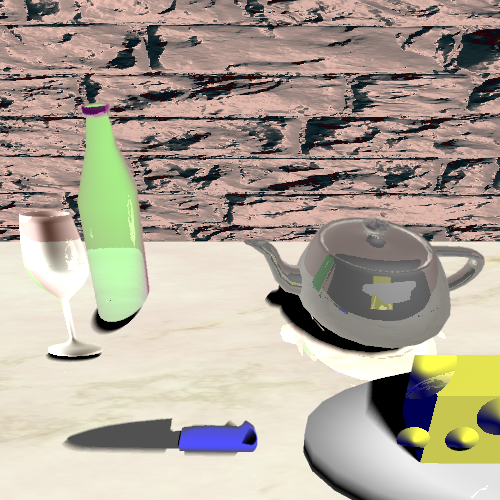
\includegraphics[width=3in]{screenshot.png}   %%%% Change file.png to your image
% \includegraphics[height=2in]{image2-FRONT.png}   %%%% Change file.png to your image
\end{minipage}


\subsection*{Artistic Merit (Polish/Artistry/Humour)}
\vfill
\subsection*{Technical Merit (Algorithms/User Interface/Graphics Techniques)}
\vfill
\subsection*{Difficulty}
\vfill
\subsection*{Code/Documentation/Demo}
\vfill
\subsection*{Mark}
\begin{center}
\begin{tabular}{lr}
Objective Mark: &~~/10\\
Subjective Mark: &~~/10\\
\hline
Total &~~/20
\end{tabular}
\end{center}

\newpage

{\huge \bf 
	\projecttitle 
}

\medskip
Name: \myname \\ 
User ID: \myuserid \\ 
Student ID: \mystudentid 

\bigskip
{\Large Objectives}

\hrule
\begin{description}
    \item[\_\_\_ 1:]  Mirror reflections on at least one object

     \item[\_\_\_ 2:]  Refraction on at least one object

     \item[\_\_\_ 3:]  Phong shading on objects

     \item[\_\_\_ 4:]  Adaptive supersampling for antialiasing

     \item[\_\_\_ 5:]  Texture mapping on at least one object

     \item[\_\_\_ 6:]  Bump mapping on at least one object

     \item[\_\_\_ 7:]  Soft shadows

     \item[\_\_\_ 8:]  Constructive solid geometry used for at least one object

     \item[\_\_\_ 9:]  Unique scene is portrayed in the image

     \item[\_\_\_ 10:]  One animation of "fuzzy" or "gaseous" object by modelling with particle systems
\end{description}

\hrule

\end{document}
